\documentclass[a4paper,10pt]{article}

\usepackage[margin=2cm]{geometry}
\usepackage{graphicx}
\usepackage{amsmath}
\usepackage{array}
\usepackage{hyperref}
\usepackage[all]{hypcap}
\usepackage{listings}
\lstdefinestyle{TerminalStyle}{
  language=bash,
  basicstyle=\small\sffamily,
  numbers=left,
  numberstyle=\tiny,
  numbersep=3pt,
  frame=tb,
  columns=fullflexible,
  linewidth=0.9\linewidth,
  xleftmargin=0.1\linewidth
}
\lstdefinestyle{HtmlStyle}{
  language=html,
  basicstyle=\small\sffamily,
  numbers=left,
  numberstyle=\tiny,
  numbersep=3pt,
  frame=tb,
  columns=fullflexible,
  linewidth=0.9\linewidth,
  xleftmargin=0.1\linewidth
}
\lstdefinestyle{OutputStyle}{
  language=html,
  basicstyle=\small\sffamily,
  frame=tb,
  columns=fullflexible,
  linewidth=0.9\linewidth,
  xleftmargin=0.1\linewidth
}

\setlength{\parindent}{0pt}
\setlength{\parskip}{1ex plus 0.5ex minus 0.2ex}
\title{
\includegraphics[width=12cm]{Eeufeeslogo.jpg} \\
       Department of Computer Science \\
       University of Pretoria \\
       \vspace{0.5cm}
       Software Engineering\\
       COS301 Main Project \\
       \vspace{0.5cm}
       \begin{large} \textbf{Team CodeX}\\ ReRoute Systems\end{large}}

\date{} 
\author{	Bondjobo, Jocelyn 		13232852 		\\
		Malangu, Daniel		13315120		\\
		Kirker, Tim			11152402		\\
		Hammond, Eunice		13222563		\\
		Burgers, Heinrich		15059538		\\
}

\begin{document}
\maketitle
\thispagestyle{empty}
\clearpage

\newpage
\pagenumbering{roman}
\thispagestyle{empty}
\tableofcontents
\clearpage

\newpage
\pagenumbering{arabic}

\section{Introduction}

	\subsection{Background} 
	Reroute Systems is a software company with different in-house developed applications. The Purchase Management System application is the main application and mainly active in the 		pharmaceutical space. The main functionality of the system is routing of request for products from account holders to the various wholesalers / suppliers, receiving the result of the order and route answer back to account holder.
	\subsection{Purpose} 	
	For the account holder to request a product he/she must search for it against the database with all the product information, the challenge is that each wholesalers / suppliers can name/describe the product differently and when the account holder do the search against the master product list the same product must be displayed across all wholesalers / suppliers using the link between master product list and the different wholesalers / suppliers product list (the user compare the prices of same product across the wholesalers / suppliers before making a decision)
	\subsection{Scope} 
	The core of the system is a search engine which is enriched with functionality
of performing some machine learning in order to retrieve the product in a master file found in a Databased running on the server through http calls. The high level modules and their responsibilities are shown in the figure below. \\ \\
	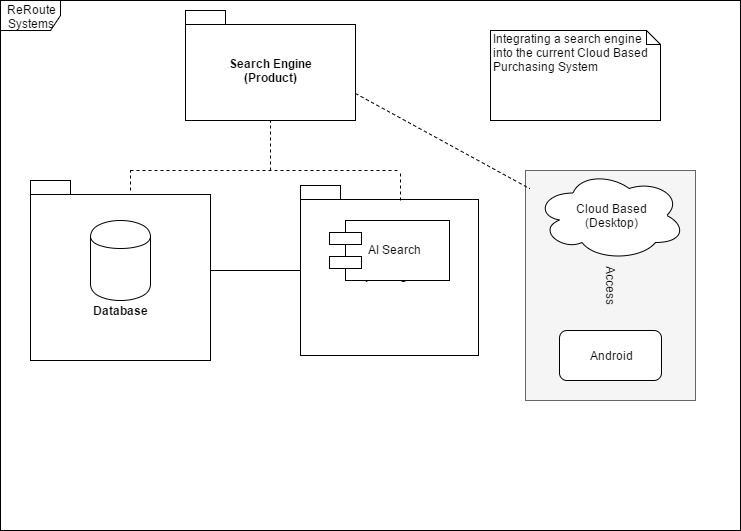
\includegraphics[scale=0.62]{scope1.jpg}
	\subsection{Definitions, Acronyms, and Abbreviations} 
	\begin{itemize} 
	\item Cloud-based : refers to applications, services or resources made available to users on demand via the Internet from a cloud computing provider's servers.
	\item Android : Mobile Operating System that allows the mobile phone to operate and install different apps in it.
	\end{itemize}
	\subsection{References} 
	\begin{itemize} 
	\item Cloud-based : refers to applications, services or resources made available to users on demand via the Internet from a cloud computing provider's servers.
	\item Android : Mobile Operating System that allows the mobile phone to operate and install different apps in it.
	\end{itemize}
	\subsection{Overview} 
	The Purchase Management System application is the main application and mainly active in the pharmaceutical space and called \textbf{Smart Rep} that can be found on Google Play store. It allows to place orders of product through mobile devices such as Android and also through Desktop as it is a cloud based system. This system monitors the routing of orders from devices to the server to different wholesalers and bring back the result.
\section{Overall Description}

\section{Overall Description}

\subsection{Product Perspective}
        \subsubsection{System Interface}{
User Interface:
\\\\
Functionality:
\\\\
The functionality of the user interface is to allow the user to interact with the system. Through this aspect of the system the user can perform all the functions necessary to use Reroute Systems. Through this the user is able to login and register an account,manage their accounts and xearch for different products.
\\\\
How functionality achieves requirements:
\\\\
The user interface allows the functionality of the application to meet the requirements. The user is able to search for any product based on any value they enter int. The user is able to be displayed information of products, that closely based o key words and values or any thing resembling the name. 
\\\\
Hardware Interface:
\\\\
Functionality:
\\\\
The functionality of this system interface is the physical hardware that allows software operation. The hardware in this case is specifically the mobile devices on which the apps run and the computers the website s usually accessed through.
\\\\
How functionality achieves requirements :
\\\\
This hardware will allow the achievement of the requirements by facilitating the operation of the application. The user will be able to press the physical device screen in order to use the search capabilities and other features of the application. The networking hardware of the components such as the wireless fidelity infrastructure or LAN connections within the devices which will allow for communication to the system server.
\\\\
Software Interface:
\\\\
Functionality:
\\\\
The functionality of the software interface is to facilitate the communication between the hardware infrastructure of the devices running the application front-end and Reroute Server. An example of this would be the operating system of the device in use. The operating system would allow the application to make use of the networking infrastructure and communicate the necessary information to the application. This would enable the device to communicate with the server and perform the necessary requests.
\\\\
How functionality achieves requirements :
\\\\
This would allow the achievement of the requirements as the communication of the application to the system server is vital to the operation of the ReRoute system. By allowing communication over WI-Fi the user is able to comunicate to the server from any location  or just stick to older and more familar devices such as computers, fulfilling the this requirement .}

		
            \subsubsection{User Interface}
	    {All users will have access to the ReRoute system when the application is launched.
For the account user interface, the registered userswill be able to login to their account, using their account information.
Their account will be used to set some of their search parameters.\\\\
}

\subsubsection{Hardware Interface}
		{
The actual Wi-Fi interface between the mobile device / computer and Wi-Fi will be abstracted by the phone and will be managed by the actual underlying operating system on the phone. On a computer the LAN interface may also be abstracted by the computer and will be managed by the actual underlying operating system on the computer if a wired connection is to be used.}
            \subsubsection{Software Interface}
            \subsubsection{Communications Interface}
	 \begin{itemize}
	    \item Users using the web will use HTTP/HTTPS protocol.
	    \end{itemize}
            \subsubsection{Memory}
	    {The mobile application will use a minimum amount of space of roughly 300MB.  the size could dramtically increase due to caching and storage of tof data locally. For the web browser the size will depend solely on caching. \\
Primary memory(RAM) will use 350MB on average, based on how long the application is being used.}
            \subsubsection{Operations}
            	{The user will require a series of normal and special case operations to be fulfilled by the system. The user will use the system in normal case operations that comprise of searching on any of the different properties of a product. On a noral case the user will search for a product based on the name of the product of interest .\\\\
            	The system will provide a registered user the option to either save there data, such as preferences, locally on the device or remotely on the server.}
           \subsubsection{Sit Adaption Requirements}
        
		\subsection{Product Functions} {The main function of the ReRoute will be to retrieve product iformation based on the values given to the user. The basic functions will include:  }
	\begin{itemize}
  		\item A search based o a specific property of a product
		\item A list of product genrics
	\end{itemize}
    	\subsection{User Characteristics}  
		{ 

There will be two main types of users interacting with the system, namely a general user and an admin. Each of these types will have different rights and access to the system and thus their own requirements.\\\\}

{The general user will use the system to retrive product information. They will need minimal skill in order to utilise the application, including the ability to connect to the Wi-Fi and use . The general user will have restricted usage of the in-app game and certain privileges that require a user profile. They will not require any additional expertise or education to function the application.\\\\}

{The Admin user will require additional permissions in order to create and update the different supplier accounts they are registered on. They will need a higher level of expertise to correctly . They will need minimal education but rather a general knowledge of the official business information.\\\\} 
    	\subsection{Constraints}   
    	\subsection{Assumptions and Dependencies}

	\section{Specific Acquirements}
This section gives a detailed description of the system requirements. It describes all the functional as well as the quality requirements of the system.

	\subsection{External Interface Requirements}

                 \subsubsection{User Interfaces}

                 \subsubsection{Software Interfaces}
The application will run on the Android operating system, specifically version 4.0. and upwards.It will also run on iOS operating system version 7.3 and above.

	\subsection{Functional Requirements}
	\subsubsection{Use case prioritization} 
		\begin{enumerate} 
		\item \textbf{Critical} 
			\begin{itemize} 
				\item Login
				\item Retrieve Wholesalers Accounts 
				\item Search Product 
				\item Logout
			\end{itemize} 
		\item \textbf{Important} 

		\item \textbf{Nice to have} 
		\end{enumerate} 

	\subsection{Performance Requirements}

	\subsection{Design Constraints}

	\subsection{Software System Attributes}

	\subsection{Other Requirements}

\subsubsection{Quality requirements}

\clearpage

\section{Open Issues}
\subsection {GitHub Repository}

\includegraphics[width=12cm]{CodeX_logo.jpg} \\
Team CodeX Repository: \url{https://github.com/josephbondjobo/CodeX}

This repository contains:
\begin{itemize}
\item All work done by team members.
\end{itemize}



\newpage
\clearpage
\addcontentsline{toc}{section}{References}

\end{document}
